\documentclass[letterpaper,twocolumn,12pt]{article}
%\usepackage{verbatim}
\usepackage[]{graphicx}
\title{Classifying Protein Secondary Structures through Deep Network Learning}
\author{Stephanie deWet and Adam Vail}

\begin{document}
\maketitle

\begin{abstract}
Classifying the secondary structures of proteins is a well-known problem in molecular biology.
Our goal is to explore the potential of applying deep learning methods to this domain.
We performed an empirical evaluation of deep network parameters on a network of stacked autoencoders.
We found that our best performance of 53.2\% resulted from parameters of window size 13, 6 hidden layers, and 26 units per hidden layer.
Unfortunately, this underperforms as compared to other learning methods.
\end{abstract}

\section{Introduction}
\label{subsec:intro}
Predicting the underlying 3D structure of a protein from its amino acid sequence is a significant problem in structural molecular biology.
An important subproblem of this is to predict complex local structures, or secondary structures, from the amino acid sequence.  
The secondary structure problem has been attacked in a variety of ways, including with x-ray crystallography, biophysical models, and machine learning models.

Within the field of machine learning, a variety of methods have been applied over the past twenty years, with varying results. 
Early work was done using standard neural networks with zero or one hidden layers resulting in the vast majority falling below 70\% accuracy.
The recent rise in popularity in deep networks (i.e. neural networks with multiple hidden layers) led us to investigate their accuracy in this problem space.

The common method of encoding amino acids uses large input vectors with an extremely sparse 1-of-k representation.
Deep networks have the ability to reduce the dimensionality of large sparse feature spaces and are potentially well suited to simplifying the secondary structure problem.

\section{Related Works}
\label{subsec:relatedworks}
One of the earliest studies in this field was conducted by Qian and Sejnowski \cite{Qian} in 1988.
They used perceptrons and standard back-propagated single hidden layer neural networks to achieve results of 63.4\% accuracy, providing us with a reference point for our baselines.

Stolorz et al. combined perceptrons with Bayesian methods to probabilistically inject domain knowledge into their model \cite{Stolorz}.
The combination of these two methods yielded an improvement over Qian with an accuracy of 64.4\%.

Rost and Sander experimented with more complex network structures similar to deep networks \cite{Rost}.
They created an ensemble of complex networks consisting of two layers of standard single hidden layer neural networks, with the output of the first being the input of the second.
Within the ensemble, each network was trained using varying parameters in order to create separation between the models.
A majority vote was used to produce the final output which was modified in special cases using specific domain knowledge.
This method produced a significant increase in performance, achieving 70.8\% in accuracy.

\section{Method}
As alluded to in section \ref{subsec:intro}, our hypothesis is that a deep network has the ability to outperform a standard neural network on the protein secondary structure classification
problem.
Our objective is to find the optimal tuning of the deep network to yield the best predictive accuracy.

\subsection{Deep Networks Consisting of Stacked Autoencoders}
We choose a standard approach to creating a deep network by stacking varying numbers of autoencoders \cite{Hinton}, which feed into a set of output units.
An autoencoder is a neural network with a single hidden layer that is trained using backpropagation to reproduce its inputs as outputs.
When there are less hidden units then inputs, the autoencoders enforce a more compact representation of the feature vector.
Our deep network consists of a set of stacked autoencoders trained using stochastic gradient descent where each successive autoencoder's inputs are the previous autoencoder's hidden layer.

\subsubsection{Input Encoding}
The training data consists of a set of proteins, each of which is a variable length sequence of amino acids.
Each amino acid in the chain can take on one of twenty discrete values.
Therefore, there are two issues that must be overcome to use an amino acid sequence as input to a neural network: handling variable length inputs and modeling discrete values.

We model the discrete values by using a 1-of-k encoding.
Each amino acid is represented by twenty input nodes, one for each of its potential values.
Of the twenty input nodes, we set the input node corresponding to the amino acid's value to one and set all others to zero.
This was chosen because we did not want to impose an ordering on the values of the amino acid or to make certain values look artificially closer to each other.
Rost and Qian chose a similar encoding.

In order to handle variable length inputs and the fact that protein sequences tend to be quite long, we chose to use a sliding window over the sequence.
For every sliding window the goal is to classify the secondary structure of the amino acid at the center of the window.
Changing the window size affects the impact of neighbors on the central amino acid's classification.
This sliding window technique was also used by Rost and Qian.

The challenge of using a sliding window is handling the amino acids that reside within half the window size of either end of the sequence.
We have chosen to model the ends of the sequence by setting each nonexistent (due to being off the end of the sequence) amino acid's twenty input nodes all to zero.

\subsubsection{Output Layer}
Our three classifications are the coarse secondary structures: alpha helix, beta sheet, and loop (also known as coil).
We represent each of these possibilities with an output unit, where the highest value of the three output units is chosen in a winner-take-all fashion.
These outputs are attached to the hidden layer of the final autoencoder, and the resultant perceptrons are trained with back propagation using stochastic gradient descent.
We use a sigmoid activation function for all units throughout the network.

\subsection{Modifications to the Basic Algorithm}
\label{subsec:mods}
We have run some tests with each of the following modifications to the deep network.

\subsubsection{Decaying hidden layer size}
The input is a large sparse array, therefore a more compact representation is desirable.
We use a decay factor to decrease the size of each stacked hidden layer, rapidly reducing the size of the feature space.

\subsubsection{Additional Connections to Output Units}
Due to the fact that the autoencoders find a compact representation of the data, we wanted to evaluate whether we were losing valuable information in the hidden layers.
The output layer was modified to take all other units in the network as input.
The final layer was then trained as a giant perceptron and continued to use a winner-take-all final predication.

\subsection{Baseline}
All related work in section \ref{subsec:relatedworks} used domain knowledge that is unavailable to us, therefore we developed our own baseline model for comparison to our deep network.
The baseline is a standard neural network using a single hidden layer and trained with back propagation using stochastic gradient descent.

\subsubsection{Ensemble of Neural Networks}
The accuracy gained by Rost from the use of an ensemble inspired us to use an ensemble as well.
We used bagging at a protein granularity to create unique training sets for each separate model.
A majority vote on the outputs of the individual neural networks was used to determine the final output.
Unfortunately, due to the time complexity of convergence and limitations of physical compute resources, we were only able to develop this for the simpler baseline neural network.

\subsection{Verification}
\label{subsec:verification}
All code for the baseline neural network and the deep network was verified by hand using small examples (amino acid sequences of length less than five).
Specifically, we traced examples through a perceptron, standard single hidden layer neural network, autoencoder, and stacked autoencoders verifying their correctness.
After many hours of debugging, we are confident the functionality of our learners are correct. 

We found that the small examples that were used for verification consistently required at least 1500 iterations over the small set of training data in order for the weights to converge.
Also, if the hidden layer size was too small, each layer may converge, but the representation would be too compact for the full network to accurately predict the structure.

\section{Empirical Evaluation}
As discussed in section \ref{subsec:intro}, the parameters we can optimize are sliding window size, hidden layer size, and number of hidden layers.
We constructed experiments to evaluate various settings of these parameters using both the deep network and the baseline neural network.
Due to the fact that the baseline consists of a single hidden layer, it converges more quickly than the deep network.
Therefore, we used results from the baseline to inform our choices of initial parameter settings when testing the deep network of autoencoders.
The basic algorithm modifications described in \ref{subsec:mods} were then evaluated using the best parameter settings from the other experiments.

\subsection{Dataset}
We chose to use a combination of the datasets created by Rost and Qian because they were curated with significant domain knowledge.
Qian's dataset is currently hosted by the University of California - Irvine's (UCI) Machine Learning Repository \cite{uci}.
We used this data without any modification as it was already divided into a 91 protein training set and a 15 protein test set.
While the test set is somewhat small, it results in approximately 3500 windows of size 13.
The Rost data consists of a total of 124 proteins.
Unfortunately, the exact data is not hosted for public use.
Therefore, we gathered the listed proteins and their corresponding labels using the Define Secondary Structure of Proteins (DSSP) database \cite{DSSP} \cite{DSSP2}.
We followed the procedure in \cite{Rost} to group the eight secondary structure classes provided by DSSP into the three standard classes mentioned previously.
We combined all proteins from Rost with Qian's training proteins to create our training data set.

Our parameter tuning experiments were tested using internal seven- or five- fold cross validation on the training dataset.
Earlier experiments used seven folds, but we switched to five-fold cross validation later due to time complexity.
After we chose our parameter values, our final experiments were trained on the entire training set and then tested on a held-aside dataset consisting of Qian's test proteins.
All plotted points in the following experiments are the average of the accuracies of each fold of the cross validation.

\subsection{Baseline Window Size}
Window size is important since it determines the number of neighbors that can influence an amino acid's classification.
Figure \ref{fig:baseline_window_size} shows that a window size of 13 or 17 is better than a smaller window.
This is to be expected, because a larger window uses results from sets in a larger neighborhood around the central amino acid.
However, increasing the window size sharply increased the number of weights that needed to be trained.
As a compromise between accuraccy and performance, we chose to use a window size of 13 for all other experiments.

\begin{figure}[ht!]
\centering
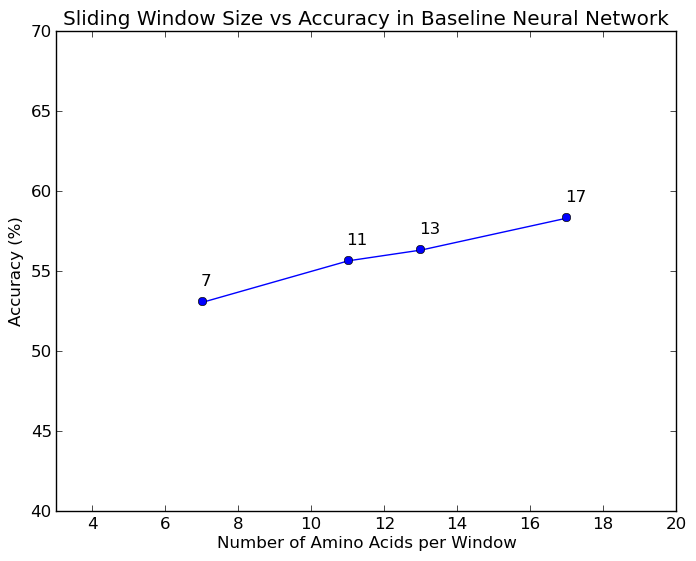
\includegraphics[width=65mm]{results/baseline/baseline_windowSize.png}
\caption{The effect of window size on accuracy, using a standard neural network. A window size of 13 was chosen for moving forward.}
\label{fig:baseline_window_size}
\end{figure}

\subsection{Baseline Hidden Layer Size}
Hidden layer size determines the degree of compaction of the new representation of the inputs.
Figure \ref{fig:baseline_hidden_layer_size} shows that fewer units in the hidden layer provides a better representation of the data.
This shows that because the input data is extremely sparse, an entire window of amino acids can be encoded in very few hidden nodes.
Due to time complexity and physical computing resources, we couldn't test any networks with more than 200 hidden units, and could only test a handful of networks with more than 100 units.
Also, we did not test any networks with size less than the window size.
Regardless, the data show that smaller numbers of hidden units per layer provide better predictive accuracy.
Based on these results, in subsequent experiments, we do not use more than 50 hidden units per layer.

\begin{figure}[ht!]
\centering
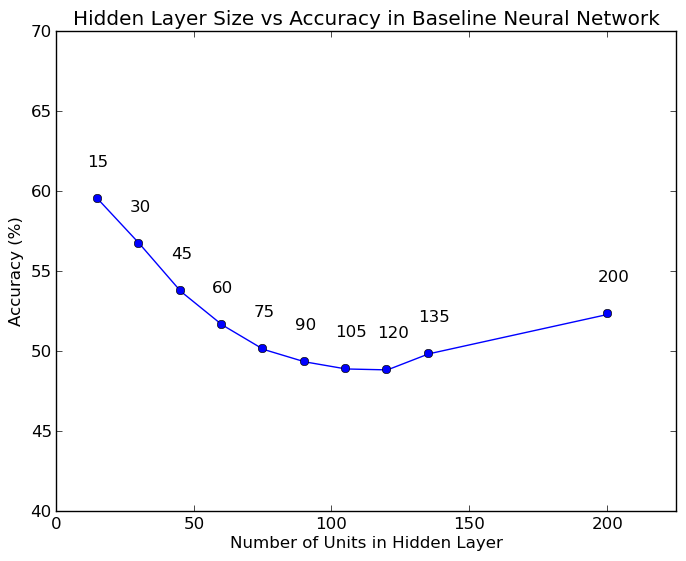
\includegraphics[width=65mm]{results/baseline/baseline_hiddenLayerSize.png}
\caption{The effect of hidden layer size, using a standard neural network.  Hidden layer sizes of less than 50 will be used moving forward.}
\label{fig:baseline_hidden_layer_size}
\end{figure}

\subsection{Best Baseline}
\label{subsec:bestbaseline}
Our best baseline network used a window size of 13 and a single 15-unit hidden layer to produce an average accuracy of 59.51\%.
Qian's parameter tuning experiments also showed that different tunings had a relatively small impact on accuracy (less than a percentage point).
Our parameter tuning experiments (for both baseline and deep network), had a similar outcome.

\subsection{Deep Network}
In deep network tests we used a window size of 13 and hidden layers sizes of less than 50.
Figure \ref{fig:deep_num_hidden_layers} shows that a larger hidden layer is necessary when stacked autoencoders are used due to the lack of network wide backpropagation.
This is consistent with the results of our single-layer neural network verification test, where a too-small hidden layer would strongly effect the network performance.
In fact, we would expect any issues in early layers to be amplified in deeper networks.
The networks with fifteen hidden units only experience small improvements with additional hidden layers.
This is unsurprising, because if information is lost in the first layer, additional hidden layers will not be able to recover it, leading to lost information in the network.

The data show that the best accuracy of 52.5\% occurs for a six hidden layer network with layer sizes of 26 units.
Without domain knowledge, it's not clear what underlying physical structure each hidden layer represents, so we are unsure why some numbers of layers work better than others.
However, the network performance consistently increases until it reaches six layers in size, after which point there is a large drop in accuracy.
We believe this is because six layers are capable of creating the most compact representation of the data the network can achieve, and additional layers simply introduce noise.

\begin{figure}[ht!]
\centering
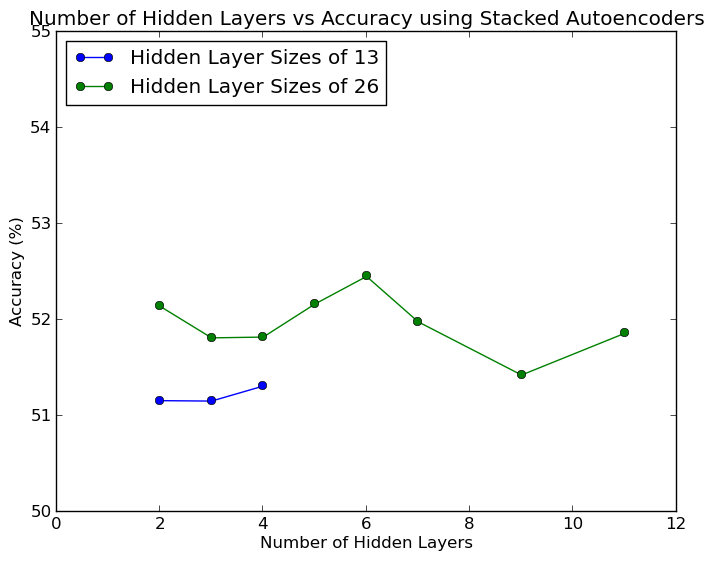
\includegraphics[width=65mm]{results/deep/numLayers/deep_numLayers.png}
\caption{The effect of hidden layer size and number of hidden layers, using a deep network. The best average accuracy (52.5\%) was achieved using 6 hidden layers with 26 units per layer.}
\label{fig:deep_num_hidden_layers}
\end{figure}

\subsection{Decay}
In all of the deep network tests until this point, the sizes of all the hidden layers in a network were the same.
We modified our algorithm to use a decay factor, so that each hidden layer was some number of units smaller than the previous layer.
The first hidden layer for these tests has 45 hidden units, so that the final layer sizes are not too small.

We found that these tests worked signifcantly worse than the standard deep networks.
With three hidden layers and a decay factor of .25, we achieved an average accuracy of 50.37\%.
With three hidden layers and a decay factor of .33, we achieved an average accuracy of 50.22\%.

We hypothesize that this is because the network is being compacted too much at each step, to the point of losing information.

\subsection{Connected Output}
In order to evaluate whether our network was losing information that was available in earlier layers, we connected the output units to every other unit in the graph.
For a network with 26 hidden units per layer and 3 hidden layers, the result was 52.20\% accuracy.
This is slightly less than the accuracy of our best deep network, with 26 hidden units and 6 layers.
That implies that the our best deep network did not lose any information between the input and final output layers.
This modification should not be used with a deeper network because it makes the final output layer very costly to train due to the explosion in size of the perceptron.

\section{Final Results and Discussion}
% Determined optimal params - now use test set too
After completing the parameter tuning experiments above, we chose optimal parameter settings.
Networks using these parameters were trained using the entire training set and tested with the held-aside test set.

\subsection{Deep Networks}
The final deep network has a window size of 13 and 6 hidden layers of size 26.
When training the final network we observed that an increase in training time significantly improved the results. 
We trained with 25, 50, and 100 iterations over the entire training set, achieving 52.26\%, 52.4\%, and 53.21\% accuracy respectively.
The 100 iteration network does almost a full percentage point better than the best parameter tuning experiment, which was trained with only 10 iterations due to the time demands of cross validation.

We created ROC curves to measure the performance of the best deep network.
Confidence was calculated by subtracting the output values for the two losing nodes from the winning output value.
Due to multiple classifications, we couldn't use the basic 2-classification ROC curve format.
Instead, we chose to use a one-versus-all ROC curve, which shows the false positive and true positive rates for each class.

\begin{figure}[ht!]
\centering
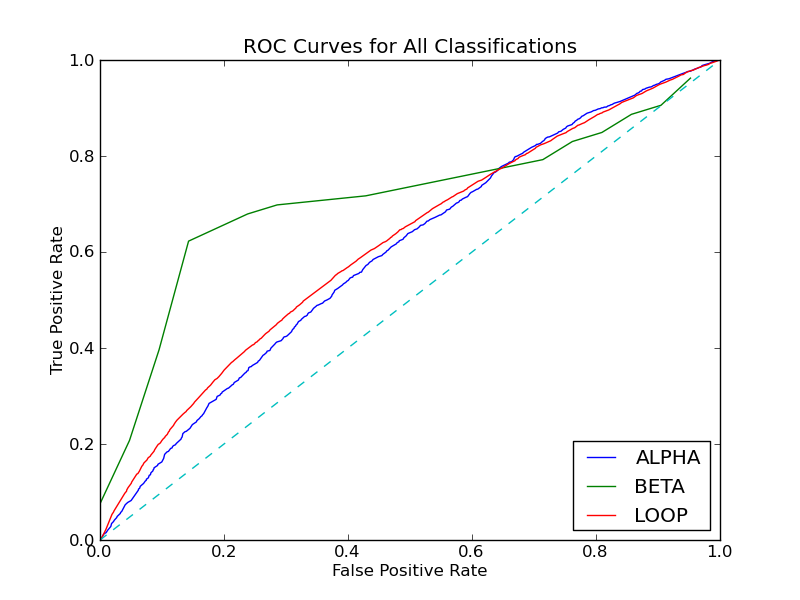
\includegraphics[width=65mm]{results/ROC_all_final_deep_net_100it.png}
\caption{ROC curves for each classification shows that the model performs better than simply guessing}
\label{fig:roc}
\end{figure}

Despite the fact that the accuracy is lower than the baseline, all three ROC curves in figure \ref{fig:roc} show that the deep network's performance is better than simply guessing.
Also note that for predictions with high confidence, our network predicts the secondary structure well, particularily beta classifications.

\subsection{Ensembles}
A natural modification to improve performance is to use ensembles of networks.
Since deep networks require significant time complexity, we were unable to train an ensemble of deep networks.
However, we were able to train an ensemble of simple neural networks with a single thirty unit hidden layer.
An ensemble of three neural networks has an average accuracy of 61.65\%.
The best baseline neural network settings, as discussed in section \ref{subsec:bestbaseline},
produced an average accuracy of 59.51\%, which is two percentage points lower than the ensemble.
Using an ensemble clearly improves the performance of the baseline network.
We hypothesize that deep networks would also benefit from this technique, but leave it to future work.

%\begin{figure}[ht!]
%\centering
%\includegraphics[width=65mm]{results/ensemble/ensemble.png}
%\caption{The effect of different numbers of neural networks on ensemble average accuracy across five runs, using standard neural networks.}
%\label{fig:baseline_ensemble}
%\end{figure}

%best baseline: 62.72
%best ensemble: 63
%best avg: 3 networks 61.65

\subsection{Final Comments on Stacked Autoencoders}
As we mentioned in section \ref{subsec:verification}, too few iterations led to a significant decrease in performance.
Due to the complexity of the data, our final deep network has not fully converged and that is why its accuracy is so much worse than the baseline.
We are confident that with significantly longer training time (on the order of weeks), the deep network would fully converge.

We still believe that deep networks have the ability to solve the secondary structure problem, but due to the time complexity of learning an effective deep network, other learning methods may be more practical.

\subsection{Lessons Learned}
In the process of working on this project, we learned that it is very difficult to understand the re-representations produced by the hidden layers of a large multi-layer network.
The combination of a complicated network and little domain knowledge made it especially challenging to tell whether these re-representations were useful.
We also learned that deep networks need to be tested very carefully, since they have so many interconnections and weights.
Overall, we feel that this was a valuable experience, gaining experience in neural networks.

\section{Future Work}
We considered additional modifications to the basic algorithm that we were unable to test due to time constraints.
We would have liked to experiment with additional functions for our hidden and output units, rather than only using a sigmoid.
One interesting modification would be using a function that further encourages sparsity by using a penalty term \cite{ng}.

\section{Conclusion}
We explored a deep network's ability to classsify secondary structures in proteins.
We created a baseline of a standard single-hidden layer neural network for comparison.
We did a parameter tuning study, and found that the best parameters for the deep network were a window size of 13 and 6 hidden layers with 26 units per layer, resulting in a final accuracy of 53.2\%.
We found that our deep networks were unable to achieve the accuracy of a standard neural network.

\begin{thebibliography}{9}


\bibitem{Hinton}
G.E. Hinton and R. R. Salakhutdinov,
   `` Reducing the dimensionality of data with neural networks"
   in \emph{Science}, 2006.

\bibitem{DSSP}
Joosten RP, Te Beek TAH, Krieger E, Hekkelman ML, Hooft RWW, Schneider R, Sander C, Vriend G,
   `` A series of PDB related databases for everyday needs"
   in \emph{NAR}, 2010.

\bibitem{DSSP2}
Kabsch W, Sander C,
   `` Dictionary of protein secondary structure: pattern recognition of hydrogen-bonded and geometrical features"
   in \emph{Biopolymers}, 1983.

\bibitem{Ng}
Andrew Ng,
   `` CS294 Lecture notes: Sparse autoencoder"
   \textbf{www.stanford.edu/class/cs294a/}
   \textbf{sparseAutoencoder.pdf}

\bibitem{Qian}
Ning Qian and Terrence J. Sejnowski,
  `` Predicting the secondary structure of globular proteins using neural network models"
  in \emph{J. Mol. Bio.}, 1988.

\bibitem{Rost}
Burkhard Rost and Christ Sander,
  `` Prediction of protein secondary structures at bettter than 70\% accuracy"
  in \emph{J. Mol. Bio.}, 1993.

\bibitem{Stolorz}
Paul Stolorz, Alan Lapedes, and Yuan Xia,
   `` Predicting protein secondary structure using neural net and statistical methods"
   in \emph{J. Mol. Bio.}, 1992.

\bibitem{uci}
   C.L. Blake and C.J. Merz,
   `` UCI repository of machine learning databases"
   \textbf{http://archive.ics.uci.edu/ml/datasets/}
   \textbf{Molecular+Biology+\}
   \textbf{(Protein+Secondary+Structure)}

\end{thebibliography}

\end{document}
